\createTitlePage{فصل سوم}{تولید جمله}
\subsection{تولید جمله}
در این بخش، به بررسی چالش تولید جمله و روش‌های پیشنهاد شده برای حل این چالش، در طول زمان، خواهیم پرداخت. در ابتدا ایده‌های اولیه در این مسیر را بیان نموده و به طور خلاصه مورد بحث قرار خواهیم داد و در ادامه به بررسی تفصیلی روش‌های مبتنی بر استفاده از شبکه‌های عصبی بازگشتی در تولید جملات زبان طبیعی، می‌پردازیم.
\\
 چالش تولید جمله، متوجه ساخت جملاتی به زبان طبیعی است، به طوری‌که از لحاظ دستور زبان، املا و معنا صحیح باشند. از طرفی با توجه به هدف اصلی ما که تولید شرح بر تصاویر است، جملات تولید شده باید علاوه بر این‌که شرط صحت مذکور را ارضا می‌کنند، با تصویر ورودی، صحنه توصیف شده در تصویر و رخ‌داد به نمایش کشیده شده، هم‌خوانی داشته باشند. تضمین این هم‌خوانی از جمله معضلات دیگری است که باید برای آن چاره‌ای اندیشید.
\\
مساله تولید خودکار جملات زبان طبیعی، یکی از مسائلی است که از دیرباز در هوش مصنوعی مطرح بوده و دارای کاربردهای فراوانی است. به عنوان یک تعریف دقیق از این مساله، می‌توان به «فرایند تولید جملات زبان طبیعی با استفاده از داده‌های غیر قابل تفسیر برای کاربران عادی در جهت افزایش قابلیت تفهیم داده‌ به آن‌ها \cite{reiter1997building}» اشاره کرد. داده‌های اولیه که جملات با استفاده از آن‌ها تولید می‌شوند، می‌توانند شامل انواع داده‌های غیر متنی از جمله نمودارها، تصاویر، اعداد و مواردی از این دست باشند.
\\
در ادامه، ابتدا کاربردهای مساله تولید خودکار جملات زبان طبیعی\enfootnote{Natural Language Generation (NLG)}، خواهیم پرداخت.


\subsection[کاربردها]{کاربردها \cite{reiter1997building}}
کاربردهای بسیار زیاد و متنوعی برای تولید خودکار جملات زبان طبیعی با استفاده از داده‌های غیر متنی، ارائه شده است. در این بخش، برای روشن شدن اهمیت این مساله، تعدادی از این کاربردها را بیان خواهیم نمود.
\\
\begin{enumerate}
\item
تولید خودکار شرح بر پیش‌بینی وضع آب و هوا با استفاده از نقشه‌های گرافیکی آب و هوا
\item 
تولید خلاصه‌ای در باره داده‌های آماری استخراج شده از یک پایگاه داده 
\item
توصیف یک زنجیره استدلالی، منتج از فرایند تصمیم‌گیری یک سیستم خبره
\item
تولید پاسخ برای پرسش‌ها در مورد یک جسم در یک سامانه مبتنی بر دانش
\end{enumerate}

موارد ذکر شده در بالا، تنها نمونه‌ای از کاربردهای وسیع این مساله در زندگی‌های روزمره را نمایش می‌دهد.

%%%%%%%%%%%%%%%%%%%%%%%%%%%%%%%%%%%%%%%%%%%%%%%%%%%%%%%%%%%
%\subsection{روش‌های مختلف موجود}


%%%%%%%%%%%%%%%%%%%%%%%%%%%%%%%%%%%%%%%%%%%%%%%%%%%%%%%%%%
\subsection{روش‌ تولید زبان طبیعی}

یکی از حوزه‌های پویا در زمینه هوش مصنوعی و پردازش متن، حوزه تولید زبان طبیعی است. این حوزه شامل فعالیت‌هایی است که به تولید جمله زبان طبیعی متناظر با داده‌های قابل تفسیر برای ماشین مانند پایگاه‌های دانش 
\enfootnote{Knowledge Bases}
و یا قالب‌های منطقی\enfootnote{Logical Forms}
و مواردی از این دست، می‌‌پردازد. روش‌های کلی که در چارچوب کاری\enfootnote{Framework}  پژوهش‌های این زمینه مورد استفاده قرار می‌گیرد، به ‌طور کلی شامل مراحل زیر است\cite{reiter1997building}.

\begin{enumerate}
\item برنامه‌ریزی متن\enfootnote{Text Planning}
\\
در این مرحله، ابتدا محتوای مورد نیاز، انتخاب می‌‌شود و چارچوب کلی برای کل متن، طرح‌ریزی می‌شود. انتخاب محتوا و طرح‌ریزی چارچوب کلی متن، با تکیه بر کاربرد مورد نظر در پژوهش و داده‌هایی که نیاز به تفسیر زبانی دارند، انجام می‌شود.
\item برنامه‌ریزی جمله\enfootnote{Sentence Planning}
\\
در این مرحله، کلمات مورد نیاز انتخاب می‌شوند، عبارات زبانی مناسب تولید می‌شوند و به طور دقیق کنارهم قرار می‌گیرند تا جملات را تشکیل دهند. انتخاب کلمات و ساخت عبارات در این بخش، بر اساس طرح کلی پی‌ریزی شده برای متن در مرحله قبل، انجام می‌شود. کنارهم قرار دادن عبارات زبانی مورد نیاز نیز، با استفاده از قواعد دستور زبان که عموما به شکل پایگاه دانش موجود است، انجام می‌گردد.
\item تحقق زبانی\enfootnote{Linguistic Realisation}
\\
در این مرحله، که مرحله نهایی است، پردازش‌های شامل پردازش‌های نحوی\enfootnote{Syntactic} برای صیقل‌دادن جملات تولید شده و تصحیح نهایی آن‌ها،‌ صورت می‌گیرد.
\end{enumerate}


اولین روش‌های ارائه شده در این حوزه، عموما محدود به کاربردهای خاص بودند. در عموم این روش‌ها، مراحل مورد نیاز برای اجرای فرایند تولید جمله به ترتیب زیر، اجرا می‌شدند.
\\
\begin{enumerate}
\item استخراج لغات متناظر با داده از طریق جدول نگاشت ثابت\enfootnote{Hardcoded Mapping Table}
\item استخراج عبارات مناسب زبانی برای تولید جمله
\item اعمال قوانین دستور زبان برای ساخت جمله
\end{enumerate}

 در \cite{reiter1997building}، روشی برای تولید جملات زبان طبیعی، بیان‌کننده وضعیت حرکت قطارها در یک ترمینال مسافربری، ارائه داده است. در این پژوهش، اطلاعات مختلف موجود در پایگاه داده، به دو دسته پیام‌های «حرکت از مبدا» و «رسیدن به مقصد» تقسیم می‌شوند و اطلاعات زمانی و شماره هر قطار در هر پیام، استخراج می‌شود. سپس با استفاده از یک جدول از پیش تعیین شده ثابت\enfootnote{Hardcoded Mapping Table}، هر پیام به یک مجموعه از لغات، نگاشت می‌شود. در ادامه، عبارات زبانی مناسب جهت تولید جملات استخراج شده و با اعمال کلیشه‌های ثابت\enfootnote{Fixed Templates} ، جملات نهایی تولید می‌شوند.

 
%%%%%%%%%%%%%%%%%%%%%%%%%%%%%%%%%%%%%%%%%%%%%%%%%%%%%%%%%%
\subsection{روش نزدیک‌ترین همسایه}

یکی از پرکاربردترین روش‌ها در این زمینه، استفاده از روش نزدیک‌ترین همسایه است. در این روش، با استفاده از بردار ویژگی‌های به دست‌آمده از داده‌های مورد تفسیر، و استخراج بردار ویژگی‌های متناظر از جملات موجود در پایگاه داده، نزدیک‌ترین جمله به بردار ویژگی حاصل، به عنوان جمله توصیف‌کننده انتخاب شده و اعلام می‌شود.
\\
پژوهش‌های زیادی با استفاده از روش نزدیک‌ترین همسایه، پردازش‌های مختلفی بر روی داده‌های متنی انجام داده‌اند. به عنوان مثال در پژوهش \cite{lawrence1995natural} با استفاده از این روش، مدلی جهت تشخیص صحت یا عدم صحت یک جمله به لحاظ دستور زبانی، ارائه شده است. در این پژوهش با استفاده از دو معیار فاصله اقلیدسی و معیار فاصله ویرایش\enfootnote{Edit Distance}، ارائه شده است. معیار فاصله ویرایش در اصل، میزان هزینه حذف، درج یا تغییر کاراکترها را در یک دنباله کاراکتری برای رسیدن به یک جمله جدید محاسبه می‌کند. مطابق با گزارش این پژوهش، بالاترین دقت به دست آمده از این مدل برای تشخیص صحت یک جمله به لحاظ دستور زبانی، برابر با $55\%$ بوده است.
\\
فعالیت‌های متعدد دیگری نیز با استفاده از این روش، سعی در شرح تصویر داشته‌اند. برای مثال در پژوهش 
\cite{hodosh2013framing}،
 ایده اصلی در تولید شرح بر تصاویر، استفاده از نزدیک‌ترین جمله به تصویر است. روش‌های مختلف و متعدد محاسبه شباهت در این پژوهش مورد بحث و بررسی قرار گرفته‌اند که به اختصار به بیان آن‌ها خواهیم پرداخت. فرض می‌شود یک مجموعه
$S_{cond}$
شامل تمام جملات موجود در مجموعه‌داده که هر کدام شرحی بر یک تصویر هستند و یک مجموعه 
$I_{cand}$
شامل تمام جملات موجود در مجموعه‌داده که هر کدام مربوط به یکی از جملات هستند، وجود دارند.

 در این پژوهش، دو هدف به طور کلی مورد نظر قرار گرفته است (در هر دو تعریف، تابع 
 $f(s,i)$
  میزان شباهت جمله $s$  و تصویر $i$ را محاسبه می‌کند). 

\begin{enumerate}
\item پیدا کردن بهترین جمله توصیف‌کننده یک تصویر
\\
در این مرحله، به دنبال یافتن $s^*$ به گونه‌ای هستیم که مقدار 
$f(s^*, i)$ 
به ازای تصویر ورودی $i$ بیشینه شود.
\item پیدا کردن بهترین تصویر توصیف‌کننده یک جمله
\\
در این مرحله به دنبال یافتن $i^*$ به گونه‌ای هستیم که مقدار 
$f(s,i^*)$
به ازای جمله ورودی $s$ بیشینه شود.
\end{enumerate}

ایده اصلی در این پژوهش، این است که با ورود یک تصویر جدید $i$ به سیستم، ابتدا نزدیک‌ترین تصویر موجود در مجموعه‌داده را نسبت به این تصویر پیدا کرده ($i^{NN}$) و سپس نزدیک‌ترین جمله به تصویر بازیابی شده ($s^{NN}$) را به عنوان جمله خروجی انتخاب می‌کنیم. برای پیدا کردن تصویر مرتبط با یک جمله نیز به همین منوال عمل می‌شود.
\\

شکل\ref{fig:knn1}
نتایج اختصاص تصاویر و جملات را توسط این روش نمایش می‌دهد. در این شکل، نتایج بصری به طور کیفی و براساس میزان خطای جمله تولیدی، به چهار دسته تقسیم شده‌اند. 


\begin{figure}[h]
\center
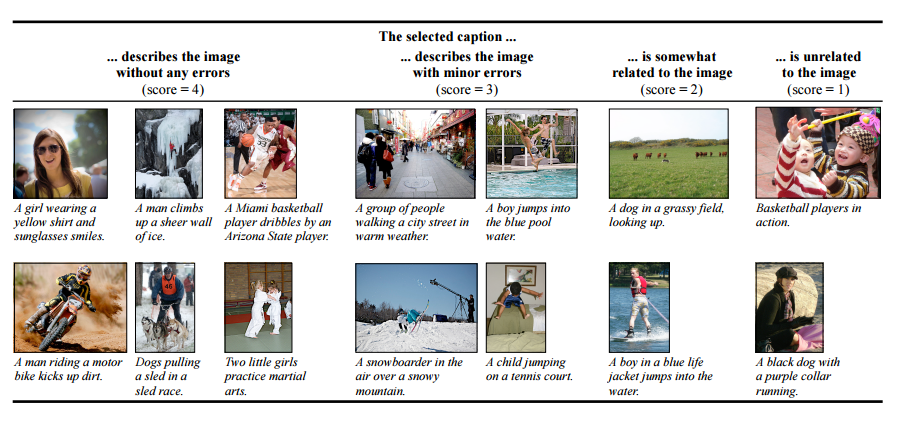
\includegraphics[scale=0.55]{Imgs/sentence_knn1.png}
\caption{نتایج کیفی اختصاص جملات و تصاویر به یک‌دیگر با استفاده از روش نزدیک‌ترین همسایه \cite{hodosh2013framing}}
\label{fig:knn1}
\end{figure}

به علاوه، جدول 
\ref{tbl:knn1}
نتایج ارزیابی روش نزدیک‌ترین همسایه را در اختصاص جملات و تصاویر به یک‌دیگر بر اساس سه معیار نمایش می‌دهد. معیار اول، میانگین امتیازی که افراد خبره به 1000 جملات تولید شده برای هر عکس داده‌اند را نمایش می‌دهد. این امتیازها اعداد صحیح بین ۱ تا ۴ را شامل می‌شوند و بیشینه ممکن برای این معیار، ۴ است. امتیاز بالاتر نشان‌دهنده مناسب‌تر بودن جملات تولید شده هستند. معیارهای \lr{BLUE} و \lr{ROUGE} معیارهایی هیتند که در پژوهش‌های ترجمه ماشین به عنوان محکی برای میزان خوب بودن ترجمه تولید شده، استفاده می‌شوند. مقادیر بالاتر در این معیارها، مناسب بودن عملکرد را نمایش می‌دهد. 

\begin{table}[h]
\center
\caption{نتایج استفاده از روش نزدیک‌ترین همسایه در اختصاص جملات و تصاویر \cite{hodosh2013framing}}
\label{tbl:knn1}
\begin{tabular}{c | c | c }
امتیاز افراد خبره & \lr{BLUE} & \lr{ROUGE}
\\
\hline
\hline
1.57 & 0.35 & 0.11\\
\end{tabular}
\end{table}

به عنوان یکی دیگر از روش‌های مورد استفاده در تولید خودکار شرح بر تصاویر، می‌توان به پژوهش ارائه شده در \cite{kuznetsova2012collective} اشاره کرد. در این پژوهش، تصاویر موجود در مجموعه‌داده، هر کدام با تعدادی عبارت زبانی که توسط کاربران انسانی نوشته شده‌اند، توصیف شده‌اند. در این پژوهش، هدف اصلی این است که با استخراج شبیه‌ترین عبارات موجود در مجموعه‌داده به تصویر ورودی و با کنارهم قرار دادن این عبارات و ساخت جمله با استفاده از چارچوب کاری مورد استفاده در پژوهش‌های تولید زبان طبیعی، جمله متناسب، تولید و نمایش داده‌شود.
\\
علاوه بر استفاده از روش نزدیک‌ترین همسایه برای انتخاب بهترین عبارات زبانی توصیف‌کننده تصویر، می‌توان از استفاده هوشمندانه از مرحله «برنامه‌ریزی محتوا»\enfootnote{Content Planning} در این پژوهش، به عنوان یکی از نقاط قوت آن، یاد کرد. این کار باعث می‌شود علاوه بر تولید جملات سازگار با یک‌دیگر، از تولید جملات تکراری در یک شرح بر یک تصویر، خودداری شود که از نقاط قوت این روش است. این مرحله با استفاده از روش‌های بهینه‌سازی انجام می‌شود. روش برنامه‌سازی خطی صحیح\enfootnote{Integer Linear Programming (ILP)}، به عنوان چارچوب کاری در این مرحله مورد استفاده قرار گرفته است.
\\
در این پژوهش، 89 کلاس از اجسام و 26 کلاس صحنه برای تشخیص محتوا انتخاب شده و تصاویر ورودی، با استفاده از آشکارکننده‌های فلزنسوالب، به این دسته‌ها اختصاص داده می‌شوند. این ‌کار، تخمین مناسبی از محتوای جملات ارائه می‌دهد. همین‌طور با استفاده از روش برچسب‌گذاری نقش کلمات در جمله\enfootnote{Part of Speech Tagging (POS Tagging)}، محتوای عبارات زبانی متناظر با جملات، به طریق مشابه، دسته‌بندی می‌شود.
\\
چهار دسته از عبارات برای هر تصویر ورودی، به این روش، استخراج می‌شود.

\begin{enumerate}
\item عبارات اسمی
\\
جستجوی عبارات اسمی موجود در مجموعه‌داده با استفاده از ویژگی بافت و رنگ به عنوان معیارهای محاسبه شباهت.
\\
مانند:
\begin{center}
\lr{
"The brown cow"
}
\end{center}
\item عبارات فعلی
\\
استفاده از معیارهای مشابه با عبارات اسمی در بین عبارات فعلی موجود در مجموعه‌داده
\\
مانند:
\begin{center}
\lr{
"boy running"
}
\end{center}
\item \enfootnote{Region/Stuff Prepositional Phrases}عبارات اضافی نواحی و اجسام
\\
جستجوی عبارات با استفاده از معیارهای شباهت رنگ، بافت، هیستوگرام گرادیان\enfootnote{Histogram of Gradient (HOG)} و همین‌طور با درنظر گرفتن ویژگی‌های هندسی اجسام
\\
مانند:
\begin{center}
\lr{
"in the sky" , "on the road"
}
\end{center}
\item عبارات اضافی صحنه\enfootnote{Scene Prepositional Pharases}
\\
جستجوی عبارات با استفاده از نتیجه دسته‌بندی صحنه با معیار $L^2$
\\
مانند:
\begin{center}
\lr{
"at the market" , "on hot summer day" , "in Sweden"
}
\end{center}
\end{enumerate}

 هر جمله شامل یک عبارت اسمی، بیان‌کننده مفعول جمله و یک یا چند نمونه از عبارتت دیگر بیان‌کننده مفهوم تصویر هستند. چهار نوع عملیات انتزاعی زیر برای ساخت جمله، در نظر گرفته شده است. هر یک از اعمال زیر با استفاده از روش برنامه‌سازی خطی صحیح، انجام می‌شوند.
 
\begin{enumerate}
 \item انتخاب مجموعه مفعولی که نیاز به توصیف دارند (هر مفعول برای یک جمله)
 \item بازچینی و ترتیب‌دهی به مفعول‌ها
 \item انتخاب مجموعه‌ عبارات مورد نیاز برای هر جمله
 \item بازچینی و ترتیب‌دهی عبارات در هر جمله
\end{enumerate}

در شکل \ref{fig:knn2}، نتایج عملکرد الگوریتم را در مقایسه با جملات تولید شده توسط انسان، مشاهده می‌نمایید. مواردی که با عبارت \lr{ILP} مشخص شده‌اند، خروجی‌های روش برنامه‌سازی خطی صحیح و مواردی که با عبارت \lr{HMM} نمایش داده شده‌اند، جملات تولید شده توسط انسان را نمایش می‌دهند.

\begin{figure}[H]
\center
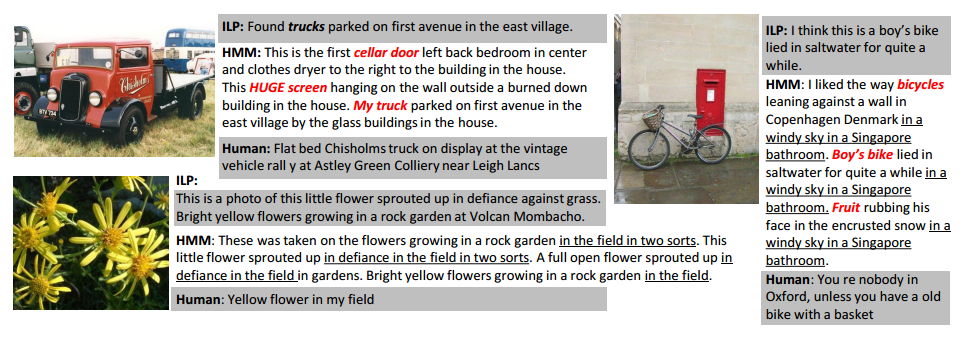
\includegraphics[scale=0.5]{Imgs/sentence_knn2.png}
\caption{نتایج برنامه‌سازی خطی صحیح در مقایسه با جملات تولید شده انسان \cite{kuznetsova2012collective}}
\label{fig:knn2}
\end{figure}

به علاوه، در شکل \ref{fig:knn3}، مواردی را مشاهده می‌نمایید که در آن‌ها، خروجی الگورتیم نسبت به جملات تولید شده توسط انسان، برتری دارد.


\begin{figure}[H]
\center
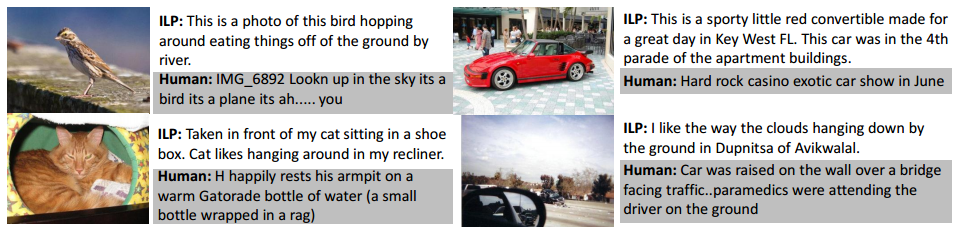
\includegraphics[scale=0.5]{Imgs/sentence_knn3.png}
\caption{مواردی از خروجی برنامه‌سازی خطی صحیح که نسبت به جملات انسان، برتری دارد \cite{kuznetsova2012collective}.}
\label{fig:knn3}
\end{figure}

با وجود این‌که الگوریتم در برخی موارد کارایی بهتری از خود نشان داده‌ است، جملاتی نیز وجود دارند که به لحاظ دستور زبان، عدم شناخت صحیح یا ناسازگاری محتوایی دچار مشکل شده‌اند. شکل \ref{fig:knn4}، نمونه‌هایی از این دست را نمایش می‌دهد.


\begin{figure}[H]
\center
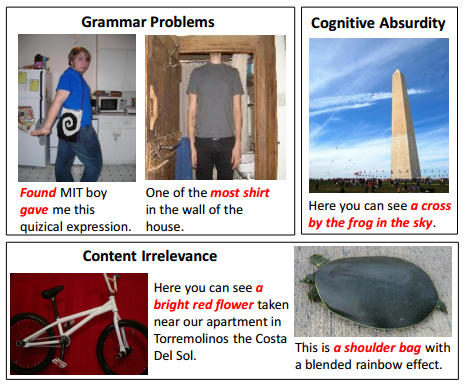
\includegraphics[scale=0.6]{Imgs/sentence_knn4.png}
\caption{نتایج برنامه‌سازی خطی صحیح که به لحاظ‌های مختلف دچار مشکل شده‌اند \cite{kuznetsova2012collective}.}
\label{fig:knn4}
\end{figure}

%%%%%%%%%%%%%%%%%%%%%%%%%%%%%%%%%%%%%%%%%%%%%%%%%%%%%%%%%%
\subsection{استفاده از قالب‌های آماده زبانی}

یکی دیگر از روش‌هایی که برای تولید جمله متناظر با یک تصویر مورد استفاده قرار می‌گیرد، روش استفاده از قالب‌های آماده زبانی است. پژوهش‌هایی که از این روش برای تولید جملات زبانی استفاده کرده‌اند، غالبا پژوهش‌های وظیفه‌‌محور\enfootnote{Task-Based} هستند. حملات تولید شده در این پژوهش‌ها عموما به طور هدف‌مند برای پاسخ دادن به موارد معینی تولید می‌شوند و قابلیت تعمیم‌پذیری کم‌تری نسبت به روش‌های دیگر دارند.
\\
به عنوان مثال در پژوهش \cite{gupta2012image}، یک روش مبتنی بر استفاده از قالب‌های آماده زبانی برای تولید خودکار شرح بر تصاویر ارائه شده است. جملاتی که در این پژوهش تولید می‌شوند، باید قادر به مشخص کردن اطلاعات زیر برای هر تصویر باشند:
\begin{enumerate}
\item اجسامی که در تصویر مشاهده می‌شوند
\item ويژگی‌های اجسام شامل رنگ، اندازه و موارد مشابه
\item فاعل
\item فعل
\item حروف اضافه
\end{enumerate}

در این پژوهش، هدف اصلی این است که پس از برجسب‌زدن تصویر با استفاده از روش‌‌های موجود در حاشیه‌نویسی تصویر\enfootnote{Image Annotation}، که در آن‌ها هر تصویر با یک یا چند برچسب زبانی حاشیه نویسی می‌شود، بتوان جمله‌های بیان‌کننده موارد فوق را در تصویر با استفاده از برچسب‌های تولید شده، تولید نمود.
در این پژوهش از مجموعه‌داده \lr{PASCAL}\enfootnote{\url{http://vision.cs.uiuc.edu/pascal-sentences/}{http://vision.cs.uiuc.edu/pascal-sentences/}} استفاده شده است که شامل 1000 تصویر و برای هر تصویر، ۵ جمله تولید شده توسط انسان است. 
\\
ابتدا با استفاده از یک ابزار برچسب‌زنی نقش کلمات در جملات، تمام کلمات موجود در جملات مجموعه‌داده، برچسب‌ زده می‌شوند. سپس برای هر تصویر، ۲ مفعول از بین ۵ جمله متناظر آن و برای هر مفعول، یک ویژگی استخراج می‌شود. به علاوه با استفاده از نرم‌افزار \lr{WordNet}، مترادف‌های هر یک از کلمات استخراج شده، تا ۳ سطح، یافت می‌شوند.
\\
در مرحله بعدی برای یافتن فاعل جمله، کافیست تعداد دفعاتی را که هر یک از ۲ مفعول استخراج شده، در بین 5 جمله موجود، در نقش فاعل بوده‌اند شمرده و کلمه‌ای را که بیشترین تعداد تکرار به عنوان فاعل را داشته است، به عنوان فاعل جمله در نظر بگیریم. با مشخص شدن فاعل و مفعول جمله، کافیست فعل مورد نظر را با شمارش تعداد دفعات تکرار افعال مختلف در جملاتی که فاعل و مفعولشان برابر با مورد در حال بررسی است، فعل با بیشترین تکرار را انتخاب کنیم. اگر چنین فعلی یافت نشد، از فعل در قالب آماده استفاده نخواهد شد.
\\
موارد مورد نیاز دیگر نیز به همین ترتیب استخراج می‌شوند. در انتها، با توجه به پیدا شدن یا نشدن فعل و همین‌طور نوع فعل استخراج شده، از یکی از قالب‌های زیر برای ساخت جمله استفاده می‌شود.
\begin{enumerate}
\item فعل اصلی استخراج شده است:
\begin{center}
(معرف ۱ - ویژگی ۱ - فاعل) - فعل - حرف اضافه - (معرف ۲ - ویژگی ۲ - مفعول)
\end{center}
\item فعل گذرا استخراج شده است:
\begin{center}
(معرف ۱ - ویژگی ۱ - فاعل) - فعل - (معرف ۲ - ویژگی ۲ - مفعول)
\end{center}
\item فعلی یافت نشده است:
\begin{center}
(معرف ۱ - ویژگی ۱ - فاعل) - حرف اضافه - (معرف ۲ - ویژگی ۲ - مفعول)
\end{center}
\end{enumerate}

شکل \ref{fig:temp1} مواردی از جملات تولید شده برای تصاویر موجود در مجموعه‌داده را نمایش می‌دهد. نمونه‌هایی که در این شکل مشاهده می‌شود، نمونه‌هایی هستند که به لحاظ معنایی صحیح بوده و با تصویر مربوطه سازگاری دارند.

\begin{figure}[H]
\center
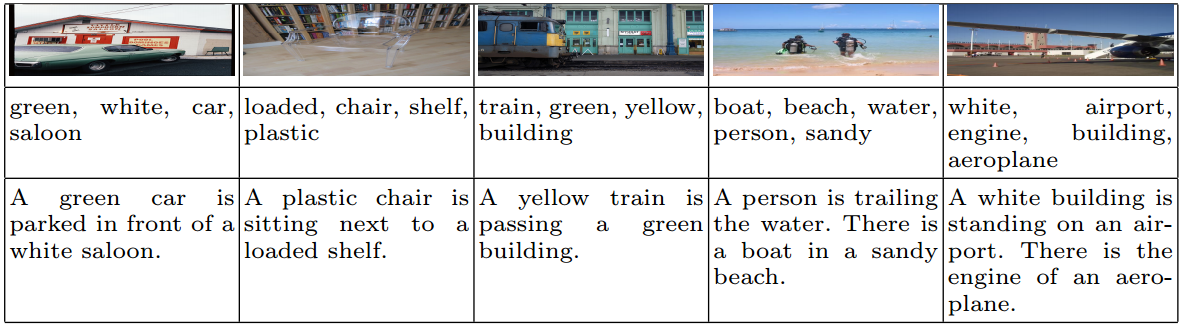
\includegraphics[scale=0.4]{Imgs/sentence_template1.png}
\caption{نمونه‌های صحیح از جملات تولید شده توسط قالب‌های آماده زبانی\cite{gupta2012image}}
\label{fig:temp1}
\end{figure}

به علاوه در شکل \ref{fig:temp2}، نمونه‌هایی از خروجی الگوریتم را در حالاتی که جملات تولید شده به لحاظ شناخت صحیح فاعل، ویژگی، فعل، حروف اضافه و همین‌طور تکرار کلمات در جمله دچار مشکل شده‌اند، نمایش می‌دهد.

\begin{figure}[H]
\center
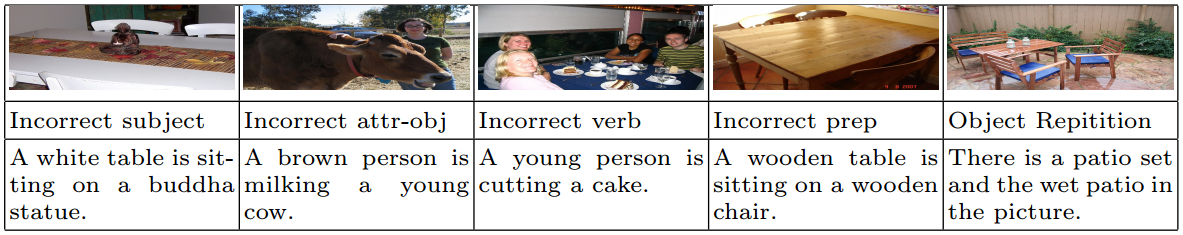
\includegraphics[scale=0.4]{Imgs/sentence_template2.png}
\caption{نمونه‌های اشتباه تولید شده توسط قالب‌های آماده زبانی\cite{gupta2012image}}
\label{fig:temp2}
\end{figure}

علاوه بر این، جدول \ref{tbl:temp1}، نتایج معیار \lr{BLUE} را در حالات مختلف (استفاده از ترکیبات چندتایی کلمات\enfootnote{n-grams}) نمایش می‌دهد. همان‌طور که مشاهده می‌شود، مقادیر به‌دست آمده از این معیارها، قابل قبول بودن دقت جملات تولید شده توسط این روش را نمایش می‌دهند. در ستون‌هایی از جدول که از حرف \lr{s} استفاده شده، تطابق بین کلمات هم‌معنی نیز در نظر گرفته شده است در صورتی‌که در بقیه ستون‌ها، کلمات دقیق با هم مقایسه شده‌اند. همان‌طور که مشخص است، استفاده از کلمات هم‌معنی نتایج بهتری را ارائه داده است.

\begin{table}[H]
\center
\caption{نتایج معیارهای \lr{BLUE} و \lr{ROUGE} درحالات مختلف \cite{gupta2012image}}
\label{tbl:temp1}
\begin{tabular}{c | c | c | c | c | c | c | c}
\lr{BLUE-1} & \lr{BLUE-1-s} & \lr{BLUE-2} & \lr{BLUE-2-s} & \lr{BLUE-3} & \lr{BLUE-3-s} & \lr{ROUGE-1} & \lr{ROUGE-1-s} 
\\
\hline
\hline
0.74 & 0.79 & 0.55 & 0.61 & 0.35 & 0.42 & 0.55 & 0.60 \\
\end{tabular}
\end{table}

%%%%%%%%%%%%%%%%%%%%%%%%%%%%%%%%%%%%%%%%%%%%%%%%%%%%%%%%%%%
%\subsection{روش‌های مبتنی بر مدل‌های آماری}
%
%%%%%%%%%%%%%%%%%%%%%%%%%%%%%%%%%%%%%%%%%%%%%%%%%%%%%%%%%%%
%\subsection{روش‌های صوری}
%
%%%%%%%%%%%%%%%%%%%%%%%%%%%%%%%%%%%%%%%%%%%%%%%%%%%%%%%%%%
\subsection{روش‌های مبتنی بر شبکه‌های عصبی بازگشتی}
اخیرا، استفاده از شبکه‌های عصبی بازگشتی برای تولید جمله، توجه تعداد زیادی از پژوهش‌گران را به خود جلب کرده است. شبکه‌های عصبی بازگشتی، ضمن اثبات قدرت خود در پیش‌بینی سری‌های زمانی، در کاربردهای متعدد و متنوعی مورد استفاده قرار می‌گیرند. از جمله این کاربردها می‌توان به تولید تصاویر، تولید متن، تولید برنامه، تولید موسیقی و مواردی از این دست اشاره نمود. با توجه به ظرفیت بالا و توان یادگیری بالای این مدل‌ها، استفاده از آن‌ها در تولید جملات زبان طبیعی مرتبط با مفهوم یا مفاهیمی خاص، نظر بسیاری را به خود جلب کرده است.
\\
شبکه‌های عصبی بازگشتی در اواخر دهه 1990، ارائه شدند و فعالیت‌های محدودی بر روی مدل‌های کوچکی از ‌آن‌ها مانند مدل \lr{Elman} انجام شد. به دلیل زمان بالای مورد نیاز برای آموزش این نوع از شبکه‌های عصبی، تا سال 2011، عموم فعالیت‌ها در این زمینه، محدود به استفاده از مدل‌های کوچک از این شبکه‌ها بودند. در سال 2011، آقای هینتون\enfootnote{Hinton} و همکارانش در پژوهش \cite{sutskever2011generating}، با بهره‌گیری از پیشرفت‌های جدید در بهینه‌سازی روش بدون هسین\enfootnote{Hessian Free (HF)} و اعمال این روش‌ها به فرایند تولید جمله در سطح حروف\enfootnote{Character Level Sentence Generation} قادر به آموزش یک شبکه عصبی بازگشتی در 5 روز شدند و نتایج بهتری نسبت به مدل‌های ارائه شده تا آن زمان، حاصل کردند.
\\
در پژوهش \cite{sutskever2011generating}، علاوه بر ارائه یک روش برای آموزش شبکه‌های عصبی بازگشتی عمیق بر مبنای روش بهینه‌سازی بدون هسین، نشان داده شده است که شبکه‌های عصبی بازگشتی استاندارد، عملکرد خوبی در تولید جملات در سطح حروف از خود نشان نمی‌دهند. برای حل این مساله، نوع خاصی از این شبکه‌ها موسوم به شبکه‌های عصبی بازگشتی عمیق ضربی\enfootnote{Multiplicative Recurrent Neural Networks (MRNN)} ارائه شده‌اند.
\\
نکات جالبی که در نتایج شبکه عصبی بازگشتی ارائه شده در این پژوهش به چشم می‌خورد، عبارتند از:
\begin{enumerate}
\item تولید ساختارهای زبانی سطح بالا\enfootnote{High level linguistic structures}
\item پشتیبانی از دایره لغات بسیار وسیع
\item یادگیری تعداد قابل توجهی از دستورات زبانی
\item تولید تعداد زیادی اسم محتمل که در بین لغات مجموعه‌داده وجود ندارند
\item توانایی باز و بسته کردن صحیح پرانتزها و نقل قول‌ها در فواصل طولانی بیشا ز 30 حرف
\end{enumerate}

یک شبکه عصبی بازگشتی را که دنباله زمانی $(x-1 \cdots x_T)$ را به عنوان ورودی گرفته و دنباله $(h_1 \cdots h_T)$ و دنباله $(o_1 \cdots o_T)$ را به ترتیب به عنوان حالات مخفی و خروجی، تولید می‌کند می‌توان مطابق با رابطه 
\ref{eq:rnn1}
بیان کرد. در این رابطه، $W_{hx}$ ماتریس وزن‌های لایه ورودی به لایه مخفی، $W_{hh}$ ماتریس وزن‌های لایه مخفی به لایه مخفی (وزن‌های بازگشتی) و $W_{oh}$ ماتریس وزن‌های لایه مخفی به لایه خروجی است. بردارهای $b$، بردارهای بایاس هستند و مقدار $W_{hh}h_{t-1}$ در نقطه $t = 1$ با یک مقدار اولیه جایگزین می‌شود.

\begin{align*}
h_t &= tanh(W_{hx}x_t + W_{hh}h_{t-1} + b_h) 
\\
o_t &= W_{oh}h_t + b_o
\numberthis
\label{eq:rnn1}
\end{align*}

از آنجا که مشتقات رابطه \ref{eq:rnn1} قابل محاسبه هستند، به راحتی می‌توان رابطه به‌روزرسانی وزن‌ها را بر اساس روش نزول در امتداد گرادیان، برای شبکه عصبی بازگشتی، محاسبه کرد. با این وجود، به دلیل رابطه بین پارامترها و دینامیک شبکه، روش نزول در امتداد گرادیان کارایی خوبی در آموزش شبکه برای پیش‌بینی دنباله‌های زمانی در بازه‌های زمانی بزرگ، ارائه نمی‌دهد. به همین دلیل، تا سال 2011 و ارائه روش بهینه‌سازی بدون هسین در \cite{sutskever2011generating} برای آموزش شبکه عصبی بازگشتی، پژوهش‌های زیادی در این زمینه انجام نمی‌شد.
\\
برای رفع مشکل روش پس‌انتشار خطا\enfootnote{Backpropagation} در آموزش شبکه‌های عصبی بازگشتی، سه روش زیر پیشنهاد شده است:
\begin{enumerate}
\item استفاده از شبکه‌های عصبی حالت پژواک\enfootnote{Echo State Network}
\\
در این شبکه‌ها، فقط وزن‌های پیش‌رو\enfootnote{Feed forward}‌ به روزرسانی می‌شوند. مقادیر اولیه برای وزن‌های بازگشتی باید به طور مناسب انتخاب شوند.
\item شبکه‌های حافظه کوتاه‌مدت بلند\enfootnote{Long Short Term Memory (LSTM)}
\\
در این شبکه‌ها، گره‌هایی برای به‌خاطر سپاری ورودی‌های قدیمی تعبیه می‌شود که باعث افزایش قدرت این شبکه‌ها در پیش‌بینی بلندمدت دنباله‌های زمانی می‌شود.
\item استفاده از بهینه‌سازی بدون هسین در آموزش شبکه‌های عصبی بازگشتی ضربی
\\
این مدل، تاکنون توانسته کارایی بهتری از هر دو مدل قبلی از خود نشان دهد \cite{sutskever2011generating}.
\end{enumerate}

در ادامه به بررسی شبکه عصبی ارائه شده در پژوهش \cite{sutskever2011generating} می‌پردازیم.

\subsubsection[شبکه عصبی بازگشتی ضربی]{شبکه عصبی بازگشتی ضربی\cite{sutskever2011ge3nerating}}

ایده اصلی در طراحی این شبکه این است که به جای استفاده و آموزش یک ماتریس یکسان از وزن‌های لایه مخفی به ازای تمام ورودی‌های ممکن، به ازای هر ورودی ممکن، یک ماتریس وزن داشته باشیم. به عبارت دیگر، هر حرفی که به عنوان ورودی به شبکه وارد شد، مشخص کننده ماتریسی باشد که به عنوان وزن‌های لایه مخفی در آموزش شبکه شرکت می‌کند. با این ایده، رابطه \eqref{eq:rnn1} به شکل رابطه \eqref{eq:rnn2} تبدیل می‌شود. 

\begin{align*}
h_t &= tanh(W_{hx}x_t + W_{hh}^{(x_t)}h_{t-1} + b_h) 
\\
o_t &= W_{oh}h_t + b_o
\numberthis
\label{eq:rnn2}
\end{align*}

همان‌طور که ملاحظه می‌شود، تنها تفاوت رابطه 
\eqref{eq:rnn1}
 و رابطه 
 \eqref{eq:rnn2}
  در بالانویس پارامتر 
 $W_{hh}$
  است. پارامتر جدید را می‌توان به شکل رابطه 
 \eqref{eq:rnn3}
  تعریف کرد که در آن، 
  $x_t^{(m)}$
   مولفه
   $m$
   ام از ورودی
  $x_t$
   و 
  $W_{hh}^{(m)}$
   است. لازم به ذکر است در رابطه
    \eqref{eq:rnn3}
     برای تعریف 
   $W_{hh}^{(x_t)}$ 
   از تنسور
   \enfootnote{Tensor}
    استفاده شده است. در این میان،
     $M$
      تعداد ابعاد ورودی 
     $x_t$
      و ماتریس‌های 
     $W_{hh}^{(1)}$
      تا 
     $W_{hh}^{(M)}$
      ماتریس‌های 
مربوط به هریک از ابعاد ورودی هستند.

\begin{equation}
W_{hh}^{(x_t)} = \ML{\Sigma}_{m = 1}^M x_t^{(m)}W_{hh}^{(m)}
\label{eq:rnn3}
\end{equation}

مدل ارائه شده از آنجا که به طور کامل عمومی است، در حالاتی که ابعاد ورودی و تعداد گره‌های مخفی زیاد باشد، دچار مشکل می‌شود زیرا حجم زیادی حافظه نیاز خواهد داشت. برای حل این مشکل، سعی در فاکتورگیری از پارامتر $W_{hh}^{(x_t)}$ خواهیم داشت.
\\
با تعریف سه ماتریس 
$W_{hf}$
، $W_{fh}$ و $W_{fx}$ و تغییر رابطه \eqref{eq:rnn3} به شکل رابطه \eqref{eq:rnn4}، می‌توان این فاکتورگیری را تعریف کرد.

\begin{equation}
W_{hh}^{(x_t)} = W_{hf} \cdot diag(W_{fx}x_t) \cdot W_{fh}
\label{eq:rnn4}
\end{equation}

در صورتی‌که ابعاد ماتریس $W_{fx}x_t$ که آن را $F$ خواهیم نامید، بزرگ باشد، رابطه \eqref{eq:rnn4} به همان اندازه رابطه \eqref{eq:rnn3} پیچیده خواهد بود اما در صورتی‌که این ابعاد کوچک باشد، رابطه \eqref{eq:rnn4} نسبت به رابطه \eqref{eq:rnn3} به مراتب ساده‌تر خواهد بود. با جای‌گذاری رابطه \eqref{eq:rnn4} در رابطه \eqref{eq:rnn2}، شبکه عصبی بازگشتی ضربی به‌دست خواهد آمد. رابطه نهایی را می‌توان به شکل رابطه \eqref{eq:rnn5} نمایش داد.

\begin{align*}
f_t &= diag(W_{fx}x_t) \cdot W_{fh}h_{t-1}
\\
h_t &= tanh(W_{hf}f_t + W_{hx}x_t)
\\
o_t &= W_{oh}h_t + b_o
\numberthis
\label{eq:rnn5}
\end{align*}

شکل \ref{fig:rnn1}
طرح‌واره‌ای از مدل کلی شبکه عصبی بازگشتی ضربی را که توسط رابطه \eqref{eq:rnn5} مدل شده است، نمایش می‌دهد. علامت مثلث که در شکل نشان داده شده است، نمایش‌دهنده یک گیت\enfootnote{Gate} را نمایش می‌دهد که در آن، وزن لایه مخفی با استفاده از ورودی، انتخاب می‌شود.

\begin{figure}[H]
\center
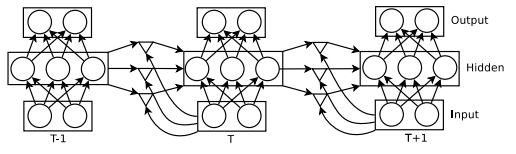
\includegraphics[scale=0.8]{Imgs/sentence_rnn1.png}
\caption{طرح‌واره شبکه عصبی بازگشتی ضربی \cite{sutskever2011generating}}
\label{fig:rnn1}
\end{figure}

نکته‌ای که هم‌چنان مبهم باقی می‌ماند، نحوه محاسبه وزن‌های مخفی است. رابطه \eqref{eq:rnn6} نحوه محاسبه $W_{hh}^{(x_t) ij}$ را نمایش می‌دهد. در این حاصل‌ضرب، اگر به عنوان مثال پارامتر $W_{hh if}$ خیلی کوچک باشد و $W_{hh fj}$ خیلی بزرگ باشد یا برعکس، حاصل مشتق، برای وزن‌های بسیار کوچک، بسیار بزرگ می‌شود و برای وزن‌های بسیار بزرگ، بسیار کوچک. این باعث می‌شود روش نزول در امتداد گرادیان، به حالت پایداری نرسد.

\begin{equation}
W_{hh}^{(x_t) ij} = \ML{\Sigma}_f W_{hh if}W_{hh fx^t}W_{hh fj}
\label{eq:rnn6}
\end{equation}

به دلیل همین عدم پایداری ایجاد شده، حاصل از رابطه \eqref{eq:rnn6}، روش نزول در امتداد گرادیان، گزینه‌ مناسبی برای آموزش این شبکه نخواهد بود. لذا لزوم استفاده از روش‌های مرتبه دوم مانند روش بدون هسین، مشهود می‌شود.

\subsubsection{تولید جمله با مفهوم مشخص}
استفاده از شبکه عصبی بازگشتی ضربی منجر به فراهم‌سازی بستری مناسب جهت تولید جمله در سطح حروف می‌شود. با این وجود برای تولید خودکار شرح بر تصاویر، نیازمند آن‌ هستیم که محتوای جملات را به طور مشخص و از پیش تعیین شده داشته باشیم. به همین دلیل نیاز به ارائه روش که طی آن بتوانیم معنا و محتوای جملات تولید شده توسط شبکه عصبی بازگشتی را کنترل کنیم، مشهود می‌شود.
\\
در پژوهش \cite{karpathy2015deep} روش جدیدی برا تولید شرح خودکار بر تصاویر ارائه شده است که در مرحله تولید جمله، از نوع خاصی از شبکه‌های عصبی بازگشتی موسوم به شبکه عصبی بازگشتی دوطرفه\enfootnote{Bidirectional RNN}، استفاده  شده است. در این روش، ابتدا از یک شبکه عصبی کانولوشنی عمیق بر روی نواحی استخراج شده از تصاویر برای استخراج ویژگی و درک صحنه استفاده شده است. از سوی دیگر، با اعمال یک شبکه عصبی بازگشتی دوطرفه بر جملات و ارائه یک تابع هدف ساختارمند، روشی برای هم‌ترازسازی جمله و اطلاعات بصری نهفته در تصویر ارائه شده است.
\\

شکل \ref{fig:deep1}، نمونه‌ای از هم‌ترازسازی ارائه شده در این پژوهش برای یک تصویر را نشان می‌دهد.
\begin{figure}[H]
\center
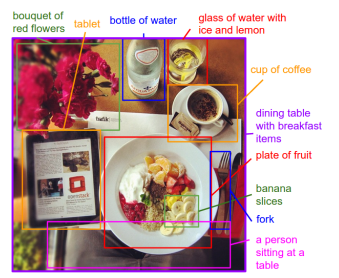
\includegraphics[scale=0.6]{Imgs/sentence_deep1.png}
\caption{هم‌ترازسازی تصویر و جمله\cite{karpathy2015deep}}
\label{fig:deep1}
\end{figure}

در مدل هم‌ترازسازی ارائه شده در این پژوهش، فرض بر این است که یک مجموعه‌داده شامل تعداد زیادی تصویر و جملات متناظر با هر تصویر وجود دارد. همین‌طور فرض دیگری وجود دارد مبنی بر این‌که بخش‌های مختلف هر جمله، به نواحی خاصی از تصویر اشاره‌ می‌کنند که موقعیت این نواحی مجهول است. از طرف دیگر اشاره این بخش‌ها به نواحی مرتبط خود در تصاویر، در بین تمام مجمو‌‌عه‌داده، تکرار می‌شود. به عنوان مثال، عبارات زبانی شامل کلمه «توپ» در تمام تصاویر موجود در مجموعه‌داده، به نواحی از تصویر اشاره می‌کنند که دارای ويژگی‌های «توپ» هستند.
\\
در شکل \ref{fig:deep2} ارتباط بین بخش‌های مختلف یک جمله و نواحی متفاوت از تصویر را مشاهده می‌نمایید. همان‌طور که در شکل مشاهده می‌شود، ابتدا برای تصاویر موجود در مجموعه‌داده و شرح متناظر با هر یک از این تصاویر، ارتباطات بین عبارات مختلف از جملات و نواحی تصاویر استخراج و یادگرفته می‌شود. در ادامه، با ورود یک  تصویر جدید و براساس ارتباطات یادگرفته شده، شرح جدید برای تصویر تولید می‌شود.

\begin{figure}[H]
\center
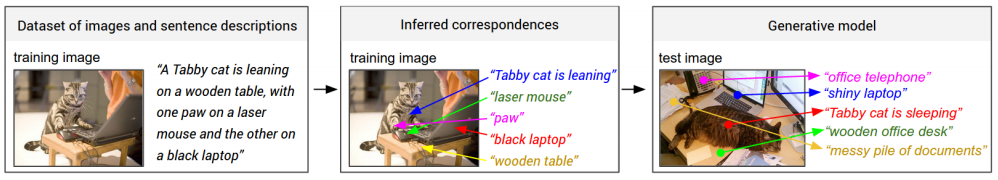
\includegraphics[scale=0.45]{Imgs/sentence_deep2.png}
\caption{ارتباط بین نواحی مختلف یک تصویر و عبارات جمله\cite{karpathy2015deep}}
\label{fig:deep2}
\end{figure}

برای تبدیل تصویر به فضای ویژگی، مطابق با آن‌چه در فصل درک صحنه ذکر شد، ابتدا با استفاده از روش شبکه‌های عصبی کانولوشنی ناحیه‌ای،‌ ۱۹ ناحیه از تصویر استخراج شده و برای ۲۰ تصویر موجود، با اعمال یک بهینه‌سازی و تخمین پارامتر و اعمال یک شبکه عصبی، بردار ویژگی استخراج می‌شود. پس از استخراج بردار ویژگی از نواحی تصویر، نیازمند آن هستیم که بتوانیم از عبارات مختلف جمله، بردار ویژگی هم‌اندازه با بردار ویژگی حاصل از تصویر، استخراج کنیم. برای این کار، در این پژوهش از شبکه‌ عصبی بازگشتی دوطرفه استفاده شده است. 
\\
این شبکه عصبی، یک دنباله از $N$ کلمه را به عنوان ورودی دریافت کرده و هر یک را به یک بردار در فضای $h$ بعدی، که $h$ اندازه بردار ویژگی حاصل از نواحی تصویر است، نگاشت می‌کند. رابطه \eqref{eq:deep1}، رابطه مربوط به پارامترهای این شبکه عصبی را نمایش می‌دهد.
در این رابطه، $I$ یک بردار ستونی اندیکاتور\enfootnote{Indicator} است که در اندیس کلمه $t$ام خود یک و در بقیه اندیس‌ها صفر دارد. $W_w$ یک ماتریس وزن ثابت برای هر کلمه $w$ است که برای جلوگیری از بیش‌برازش بر داده‌ها، مورد استفاده قرار می‌گیرد.

\begin{align*}
x_t &= W_{w} I_t 
\\
e_t &= f(W_ex_t + b_e)
\\
h_t^f &= f(e_t + W_fh_{t-1}^f + b_f)
\\
h_t^b &= f(e_t + W_bh_{t-1}^b + b_b)
\\
s_t &= f(W_d(h_t^f + h_t^b) + b_d)
\numberthis
\label{eq:deep1}
\end{align*}

 در این شبکه، دو جریان داده وجود دارد. جریان اول، جریان داده بین گر‌ه‌های مخفی شبکه از چپ به راست و دیگری جریان داده بین نود‌های مخفی شبکه از راست به چپ است که به ترتیب با $h_t^f$ و $h_t^b$ نمایش داده می‌شوند. بردار نهایی $s_t$، بردار حاصل از نگاشت کلمات به فضای ویژگی‌ها است که با استفاده از خود کلمه و محتوای مورد استفاده در اطراف کلمه در جمله، تولید می‌شود.
\\
شکل \ref{fig:deep3} طرح‌واره‌ای از معماری این شبکه را نمایش می‌دهد. همان‌طور که در این شکل مشخص است، در لایه مخفی این شبکه، دو جریان داده، یکی از راست به چپ و دیگری از چپ به راست برای محاسبه تاثیر کلمات اطراف کلمه جاری بر نگاشت کلمه به فضای ویژگی‌ها، وجود دارد.

\begin{figure}[H]
\center
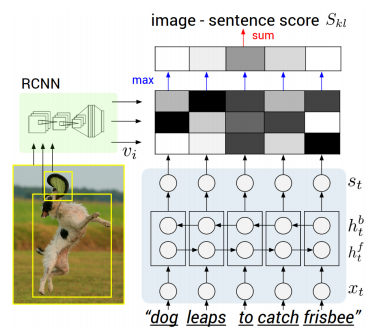
\includegraphics[scale=0.8]{Imgs/sentence_deep3.png}
\caption{طرح‌واره شبکه عصبی بازگشتی دوطرفه\cite{karpathy2015deep}}
\label{fig:deep3}
\end{figure}

 در ادامه با بهره‌گیری از روش نگاشت دوطرفه تصاویر و جملات که در بخش درک صحنه ارائه شد، توابع هم‌ترازسازی و تابع هدف ارائه شده را مورد استفاده قرار داده و با استفاده از روش یادگیری چند نمونه‌ای، اقدام به یادگیری انتساب‌های بین نواحی مختلف تصاویر و عبارات مختلف زبانی می‌شود.
 \\
 با استفاده از این روش، می‌توان برای هر ناحیه از تصویر، کلمات مناسب را تعیین کرد. اما برای تولید خودکار شرح بر تصاویر، نیاز به تولید عبارات زبانی وجود دارد. برای حل این مشکل، با در نظر گرفتن رابطه ضرب داخلی بین بردارهای ویژگی حاصل از نواحی تصویر و عبارات زبانی یک جمله به عنوان معیار شباهت، روشی ارائه شده است که بتوان برای هر ناحیه از تصویر، عبارت زبانی مناسبی تولید کرد.
 \\
 در این روش، با تعریف یک تابع انرژی و استفاده از مدل میدان تصادفی مارکف، با بهینه‌سازی تابع انرژی ارائه شده، بهترین هم‌ترازسازی برای هر یک از عبارات موجود محاسبه شده و عبارت با بهترین مقدار، انتخاب می‌شود. رابطه \eqref{eq:deep2}، این تابع انرژی را محاسبه می‌کند.
 
 
 \begin{align*}
 E(a) =  \ML{\Sigma}_{j=1\cdots N}\Psi_j^U(a_j) &+ \ML{\Sigma}_{j=1\cdots M}\Psi_j^B(a_j, a_{j+1})
 \\
 \Psi_j^U(a_j) &= \nu_i^T \cdot s^t
 \\
 \Psi_j^B(a_j,a_{j+1}) &= \beta I(a_j = a_{j+1})
 \numberthis
 \label{eq:deep2}
 \end{align*}


می‌توان در شکل \ref{fig:deep7} نتایج استفاده از این شبکه و محاسبه میزان شباهت نواحی مختلف تصویر و عبارات مختلف از جملات را مشاهده نمود. این شکل، نتیجه آموزش اختصاص نواحی مختلف تصویر به عبارات زبانی را نمایش می‌دهد.

\begin{figure}[H]
\center
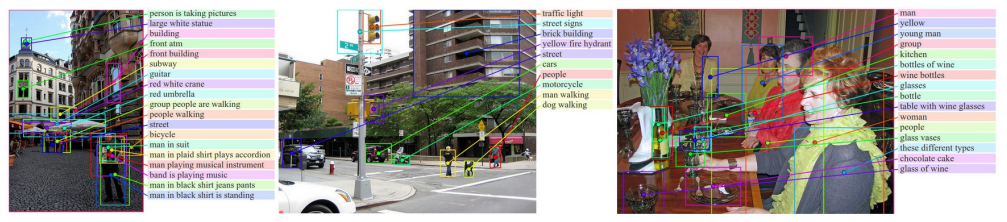
\includegraphics[scale=0.5]{Imgs/sentence_deep7}
\caption{انتساب نواحی مختلف تصویر به عبارات زبانی\cite{karpathy2015deep}}
\label{fig:deep7}
\end{figure}


تا این مرحله، با ورود یک تصویر، یا یک ناحیه از تصویر، عبارات زبانی متناظر، استخراج شده‌اند. هدف اصلی در این پژوهش تولید جمله برای هر تصویر است. بنابراین نیاز داریم تا با استفاده از مدل‌های ارائه شده برای تولید جمله، این کار را انجام دهیم. در پژوهش‌های زیادی، استفاده از شبکه‌های عصبی بازگشتی برای پیش‌بینی و محاسبه توزیع احتمال کلمه بعدی در یک جمله با در نظر داشتن کلمات قبلی و محتوای جمله، ارائه شده است. در این پژوهش با اعمال تغییرات کوچکی، از همین روش‌ها استفاده می‌شود. 
\\
رابطه ارائه شده برای شبکه عصبی بازگشتی که این کار را انجام می‌دهد، مطابق با رابطه \eqref{eq:deep3} است.
در این رابطه، $CNN_{\theta c}(IMAGE)$ بردار حاصل از اعمال آخرین لایه یک شبکه عصبی کانولوشنی بر تصویر را نشان می‌دهد و بقیه پارامترها، همگی قابل آموزش هستند. بردار $y_t$ بردار نماینده توزیع احتمالاتی تمام کلمات با در نظر گرفتن کلمات قبلی و محتوای هر ناحیه است که اندازه آن برابر است با تعداد تمام کلمات موجود در لغت‌نامه به علاوه یک نشانه خاص به عنوان «اتمام جمله».

\begin{align*}
b_\nu &= W_{hi}[CNN_{\theta c}(IMAGE)]
\\
h_t &= f(W_{hx}x_t + W_{hh}h_{t-1} + b_h + I(t = 1)\cdot b_\nu)
\\
y_t &= softmax(W_{oh}h_t + b_o)
\numberthis
\label{eq:deep3}
\end{align*}

شکل \ref{fig:deep4}، طرح‌واره‌ای از شبکه عصبی بازگشتی مالتی‌مودال\enfootnote{Multimodal} ارائه شده در این پژوهش برای تولید جمله را نمایش می‌دهد.

\begin{figure}[H]
\center
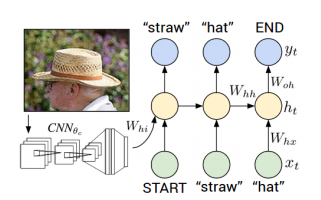
\includegraphics[scale=1]{Imgs/sentence_deep4.png}
\caption{طرح‌واره شبکه عصبی بازگشتی ارائه شده برا تولید جمله\cite{karpathy2015deep}}
\label{fig:deep4}
\end{figure}

جدول \ref{tbl:deep}
نتایج معیار \lr{BLUE} را برای روش ارائه شده بر روی سه مجموعه‌داده مختلف، نمایش می‌دهد. همان‌طور که در این جدول مشخص است، نتایج به دست آمده از این روش در مقایسه با دو روش دیگر، نتایج به نسبت بهتری بوده است.

\begin{table}[H]
\center
\caption{نتایج معیار \lr{BLUE} برای روش ارائه شده در \cite{karpathy2015deep} در مقایسه با دو روش دیگر}
\label{tbl:deep}
\begin{tabular}{c | c | c | c || c | c | c || c | c | c | c}
نام روش
&
\lr{B-1} &\lr{B-2} &\lr{B-3} &
\lr{B-1*} &\lr{B-2*} &\lr{B-3*} &
\lr{B-1**} &\lr{B-2**} &\lr{B-3**} &\lr{B-4**} 
\\
\hline
\hline
نزدیک‌ترین‌همسایه
&
ــ &ــ & ــ &
ــ &ــ & ــ &
45.0 &28.1 &16.6 &10.0
\\
روش \cite{mao2014explain}
&
58 & 28 & 23 &
55 & 24 & 20  &
ــ &ــ &ــ &ــ
\\
روش \cite{karpathy2015deep}
&
57.9 & 38.3 & 24.5 & 57.3 & 36.9 & 24.0 & 62.5 & 45.0 & 32.1 & 23.0 

\end{tabular}

\end{table}


شکل \ref{fig:deep5} نتایج رتبه‌بندی جملات و عبارات برای هر ناحیه از تصویر را نمایش می‌دهد.

\begin{figure}[H]
\center
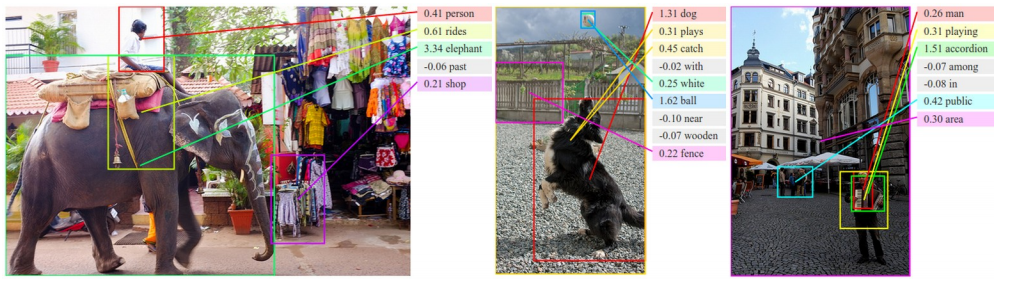
\includegraphics[scale=0.5]{Imgs/sentence_deep5.png}
\caption{نتایج رتبه‌بندی عبارات زبانی برای نواحی تصویر \cite{karpathy2015deep}}
\label{fig:deep5}
\end{figure}

به علاوه، در شکل \ref{fig:deep6} نتایج تولید شرح برای تصاویر، توسط شبکه عصبی بازگشتی ارائه شده در این پژوهش، به تصویر کشیده شده است.

\begin{figure}[H]
\center
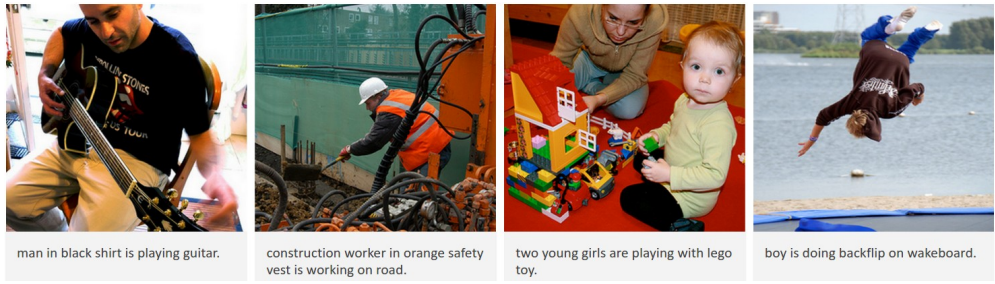
\includegraphics[scale=0.5]{Imgs/sentence_deep6}
\caption{نتایج تولید جمله برای تصاویر در \cite{karpathy2015deep}}
\label{fig:deep6}
\end{figure}



%%%%%%%%%%%%%%%%%%%%%%%%%%%%%%%%%%%%%%%%%%%%%%%%%%%%%%%%%%
\subsection{جمع‌بندی}

چالش تولید جمله یکی از قدیمی‌ترین و پویاترین حوزه‌های فعالیتی و پژوهشی در هوش مصنوعی است که از اواسط قدن بیستم، توجه پژوهش‌گران بسیاری را به خود جلب کرده است. روش‌های مختلفی برای حل این مساله ارائه شده‌اند. از جمله این روش‌ها می‌توان به موارد زیر اشاره کرد:

\begin{enumerate}
\item تولید زبان طبیعی
\\
در این دسته از روش‌ها که از اواخر دهه بیستم تا کنون مورد استفاده قرار می‌گیرند، با طی فرایند در یک چارچوب کلی، سعی در تولید جملات مناسب دارند. این دسته از روش‌ها عموما برای تفسیر خودکار داده‌هایی که برای کاربران انسانی غیر قابل تفسیر هستند یا تفسیر دشواری دارند، به‌کار می‌روند. در این روش‌ها ابتدا با استفاده از ویژگی‌های مختلفی که در داده‌های ماشینی (داده‌های قابل تفسیر برای ماشین) کلمات مناسب انتخاب شده و سپس با استفاده از کلمات منتخب، عبارات زبانی (با جایگشت دادن کلمات و حذف عبارات غیر محتمل) تولید می‌شوند. سپس با اعمال قواعد دستور زبان و چینش عبارات زبانی در کنارهم، جملات نهایی تولید می‌شوند.
\item نزدیک‌ترین همسایه
\\
در این دسته از روش‌ها سعی می‌شود با ورود یک تصویر و نگاشت آن به فضای ویژگی‌ها، جمله‌ای از میان تمام جملات موجود در مجموعه‌داده انتخاب شود که بیشترین مشابهت با بردار ویژگی تصویر را دارد. بزرگ‌ترین مشکل در این روش‌ها انتخاب معیار مناسب برای محاسبه فاصله بین یک جمله و بردار ویژگی حاصل از تصویر است. در این روش، علاوه بر این‌که نیاز به وجود مجموعه‌داده وسیع و پوشا وجود دارد، ممکن است جمله نهایی، در انتها گویا و بیان‌کننده تمام جوانب تصویر نباشد و یا حتی با تصویر ورودی سازگاری نداشته باشد.
\\
برای حل این مشکل، سعی شد به جای استخراج نزدیک‌ترین جمله به تصویر موجود، مشابه‌ترین عبارات زبانی را با شکستن جملات موجود به عبارات سازنده، انتخاب کرده و با بهره‌گیری از روش تولید زبان طبیعی و یا روش‌های دیگر، چینش مناسبی از این عبارات را که در قالب یک یا چند جمله بیان شوند، تولید و به عنوان شرح بر تصویر، نمایش داد.
\item استفاده از قالب‌های زبانی آماده
\\
با وجود فعالیت‌های گوناگون در این زمینه و استفاده از روش‌های مختلف، هم‌چنان تضمین صحت جمله خروجی، کار دشواری است. به همین دلیل، سعی شد با ارائه یک یا چند قالب زبانی آماده و از پیش تعیین شده برای جملات، مانند قالب‌های جملات خبری، صحت جملات نهایی را تضمین کرد. در این دسته از روش‌ها، ویژگی‌های مختلفی از تصویر استخراج می‌شود که هریک از این ویژگی‌ها یا همه آن‌ها در کنار هم قادر هستند نقش‌هایی مانند «فعل»، «فاعل»، «مفعول» و موارد مشابه را در جمله متناظر با تصویر مشخص کنند. با استخراج کلمات مناسب و شناخت نقش آن‌ها در جمله و جای‌گذاری هر یک از این کلمات در مکان مناسب نقشی خود در قالب از پیش تعیین شده، جمله متناظر با هر تصویر استخراج می‌شود.
\item استفاده از شبکه‌های عصبی بازگشتی
\\
اگر چه استفاده از قالب‌های آماده و از پیش تعیین شده، تا حدی مشکلات موجود را حل می‌کند اما هم‌چنان چالش بزرگ‌تری حل نشده باقی مانده است. تولید جملات جدید، استفاده از کلمات و عبارات جدید و ابتکاری به طوری‌که علاوه بر تضمین رعایت دستور زبان، بتوان معنای جمله را نیز متضمن شد، چالش بزرگی است که در این مسیر کماکان وجود دارد.
\\
استفاده از شبکه‌های عصبی بازگشتی یکی از بهترین راه‌کارهای موجود برای حل این مشکل و رویارویی با این چالش هستند. استفاده از این شبکه‌ها در اواخر قرن بیستم در بین پژوهش‌گران رواج پیدا کرد تا جایی که ناپایداری الگوریتم پس‌انتشار خطا در آموزش این شبکه، راه را برای پژوهش‌های بعدی بست. پس از ارائه یک روش مناسب برای بهینه‌سازی بدون هسین در سال 2010، روشی برای آموزش یک شبکه عصبی بازگشتی موسوم به شبکه عصبی بازگشتی ضربی بر مبنای بهینه‌سازهای بدون هسین ارائه شد و نتایج آن به طور چشم‌گیری از روش‌های موجود بیشتر بود.
\\
ارائه شبکه عصبی بازگشتی ضربی، نقطه عطفی در مسیر علم در راستای حل چالش تولید جمله به حساب می‌آید. از حدود سال 2011 به بعد، استفاده از شبکه‌های عصبی بازگشتی برای تولید جمله به پویاترین و پرفعالیت‌ترین حوزه در مسائل مربوط به تولید جمله، به حساب می‌آید.
\end{enumerate}

خانم لی و همکارانش در سال 2015، در پژوهش \cite{karpathy2015deep}، با استفاده از شبکه‌های عصبی کانولوشنی عمیق و دو نوع از شبکه‌های عصبی بازگشتی موسوم به شبکه‌های عصبی بازگشتی مالتی‌مودال و شبکه‌های عصبی بازگشتی دوطرفه، روش مناسبی برای تولید خودکار شرح بر تصاویر ارائه داده است.
\\
در این پژوهش، ابتدا با بهره‌گیری از روش شبکه عصبی کانولوشنی ناحیه‌ای، نواحی از تصویر که شامل تصویر اجسام است، استخراج شده و با استفاده از یک شبکه عصبی کریشفسکی، بردار ویژگی برای هر ناحیه محاسبه می‌شود. سپس با بهره‌گیری از یک شبکه عصبی بازگشتی دوطرفه، عبارات مختلف از جمله استخراج و بردارهای ویژگی برای هر عبارت محاسبه می‌شود. سپس با استفاده از یک تابع هدف و مدل میدان تصادفی مارکف، هم‌ترازسازی بین نواحی و عبارات زبانی صورت گرفته و مدل آموزش داده می‌شود.
\\
 در ادامه با تخمین بهینه پارامترهای موجود و با استفاده از شبکه عصبی بازگشتی مالتی‌مودال، توزیع احتمال بهترین کلمه بعدی در یک جمله با داشتن کلمات قبلی و محتوای حاصل از بردار ویژگی محاسبه شده روی نواحی تصویر، محاسبه شده و بهترین کلمه بعدی تولید می‌شود. این کار تا جایی ادامه می‌یابد که شبکه، نشانه مخصوص پایان جمله را تولید کند.
  